\section{Theoretical Analysis} \label{section:theo}


\par In this section, a theoretical analysis of the circuit shown in section \ref{introduction} was conducted. 

\subsection{Description and Important Mathematical considerations}

First, the transfer function, of the circuit was determined. Accordingly to what was learned in lectures and in the presential laboratory class, we reached the following conclusions:

\begin{equation}
T(s)= \frac{Vout(s)}{Vin(s)}=1+\frac{Zout(s)}{Zin(s)} = \frac{R1*C1*s}{1+R1*C1*s}*(1+)\frac{R3}{R4}*\frac{1}{1+R2*C2*s}
\end{equation}


We also computed the low cutoff frequency and the high cut off frequency in octave. The central frequency was also calculated. The equations used were the following:


\begin{equation}
\omega_{L}= \frac{1}{R1*C1}
\end{equation}

\begin{equation}
\omega_{H}= \frac{1}{R2*C2}
\end{equation}

\begin{equation}
\omega_{0}= \sqrt{\omega_{L} * \omega_{H}}
\end{equation}

AS requested, the input and output impedances were also calculated as follows:


\begin{equation}
Z_{in}= R1+ \frac{1}{j*\omega_{0}*C1} 
\end{equation}

\begin{equation}
Z_{out}= \frac{R2}{j*\omega_{0}*C2*(R2+\frac{1}{j*\omega_{0}*C2})} 
\end{equation}

\subsection{Final Results}
All the important results obtained are shown in the tables and in the figure bellow. 

\begin{figure}[h] \centering
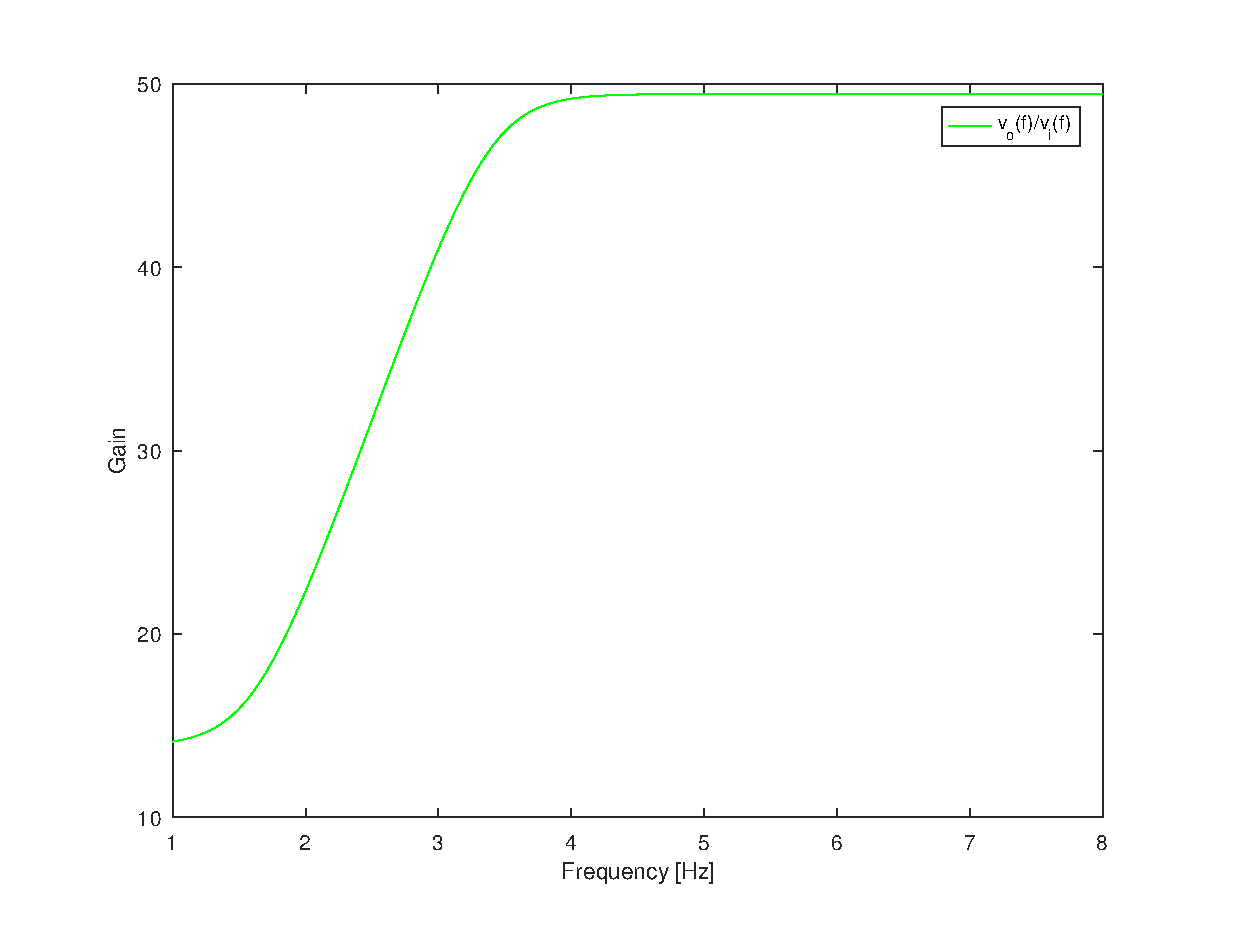
\includegraphics[width=0.65\linewidth]{theo.eps}
\caption{Voltage Gain of the circuit. Octave}
\label{sh}
\end{figure}




\begin{table}[ht]
  \centering
  \begin{tabular}{|l|r|}
    \hline    
    {\bf Name} & {\bf Value} \\ \hline
    \input{../mat/impedances_tab}
  \end{tabular}
  \caption{Input and output Impedences}
  \label{tab:2}
\end{table}



\begin{table}[ht]
  \centering
  \begin{tabular}{|l|r|}
    \hline    
    {\bf Name} & {\bf Value} \\ \hline
    \input{../mat/band_pass_freq_tab}
  \end{tabular}
  \caption{Low cut-off frequency, High cut-off frequency, Central Frequency.}
\end{table}



\begin{table}[ht]
  \centering
  \begin{tabular}{|l|r|}
    \hline    
    {\bf Name} & {\bf Value} \\ \hline
    \input{../mat/wo_freq_gain_tab}
  \end{tabular}
  \caption{Central Frequency(Hz) and Respective Gain(dB).}
\end{table}


\begin{table}[ht]
  \centering
  \begin{tabular}{|l|r|}
    \hline    
    {\bf Name} & {\bf Value} \\ \hline
    \input{../mat/Cost_Merit_tab}
  \end{tabular}
  \caption{Cost and Merit.}
\end{table}











